\begin{frame}[fragile]{Padrão borboleta para $N = 2$}

    \begin{figure}
        \centering

        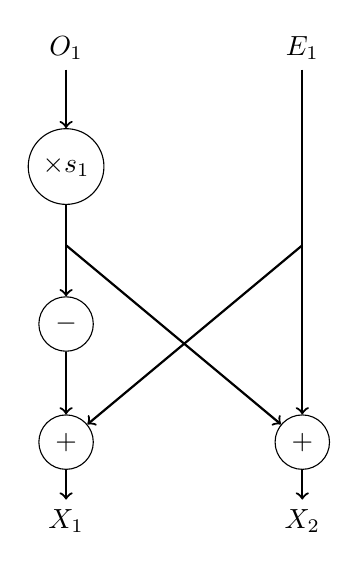
\begin{tikzpicture}
            \node (A) at (0, 5) { $O_1$ };
            \node[draw,circle] (B) at (0, 3.5) { $\times s_1$ };
            \node[draw,circle] (C) at (0, 1.5) { $\mathbf{-}$ };
            \node[draw,circle] (D) at (0, 0) { $\mathbf{+}$ };
            \node (E) at (0, -1) { $X_1$ };

            \node (F) at (3, 5) { $E_1$ };
            \node[draw,circle] (G) at (3, 0) { $\mathbf{+}$ };
            \node (H) at (3, -1) { $X_2$ };
            \coordinate (I) at (3, 2.5);
            \coordinate (J) at (0, 2.5);

            \draw[thick,->] (A) edge (B);
            \draw[thick,->] (B) edge (C);
            \draw[thick,->] (C) edge (D);
            \draw[thick,->] (D) edge (E);

            \draw[thick,->] (F) edge (G);
            \draw[thick,->] (G) edge (H);
            \draw[thick,->] (I) -- (D);
            \draw[thick,->] (J) -- (G);


        \end{tikzpicture}

    \end{figure}

\end{frame}
